\subsubsection{Outlier Identification}
An important part of the analysis of the sound files is to identify when outliers arise. Our sponsor has expressed that being able to see when an outlier occurs and being able to listen to what caused it is important in drawing conclusions and finding interesting bits of information from a data set. Thus, two infographics seem reasonable, those being timelines and line charts. Both do relatively similar jobs, however a timeline is made specifically for information over time. The only upside to a line graph would be that each point on the graph would represent a sound file, and the results of its analysis. Being able to represent an output as a small dot on a chart and allowing the user to select or hover over that point to see which file caused the outlier is certainly desirable from a usability perspective. Additionally, it would be helpful for the user to be able to select a specific sound file along with a specific time in that file and be able to listen to it on command. This feature is also included in Mangrove.\par
\begin{center}
  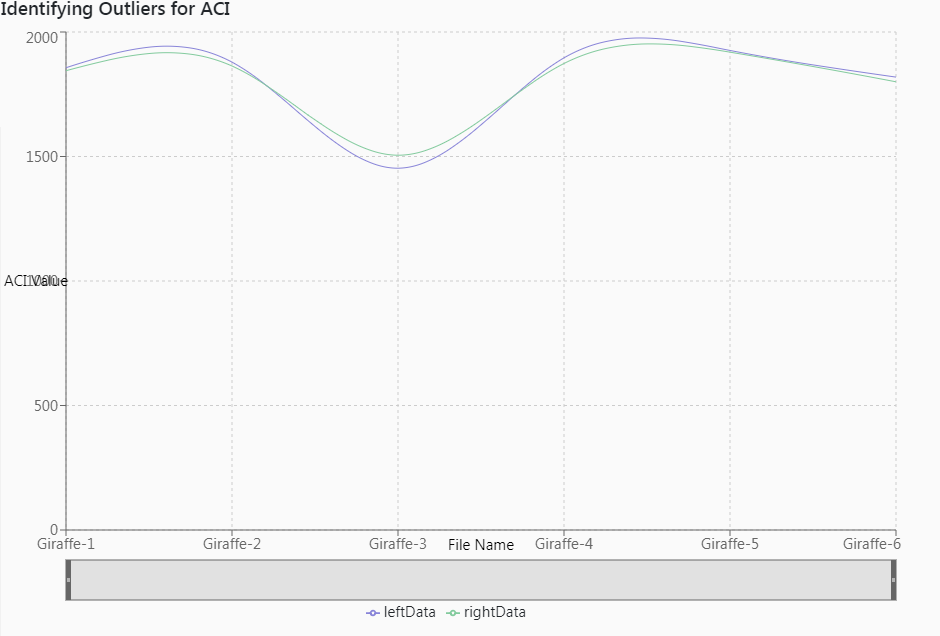
\includegraphics[width=\textwidth]{OutlierACIgraph1} \\[12pt]
  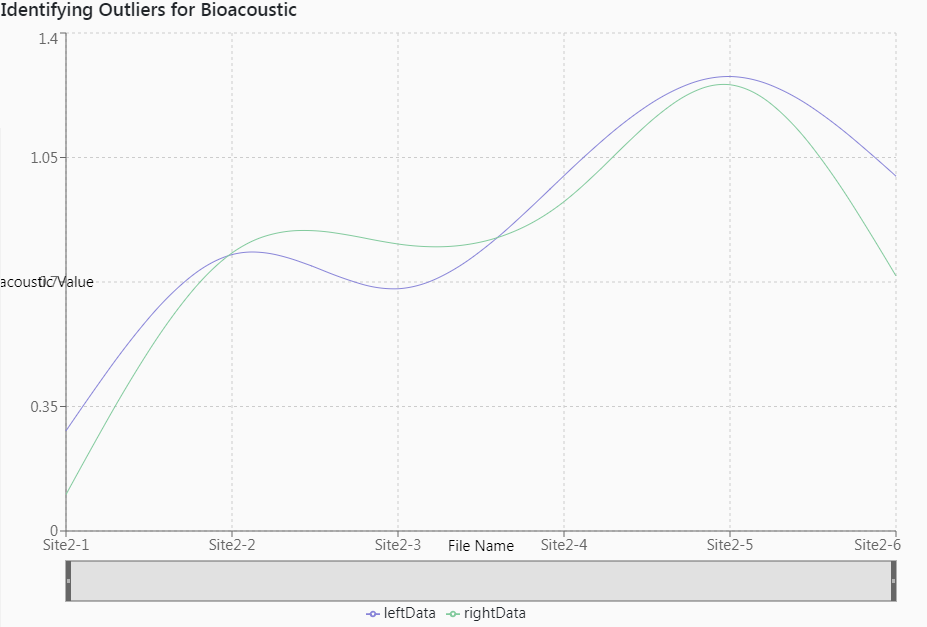
\includegraphics[width=\textwidth]{OutlierBAgraph1} \\[12pt]
\end{center}
The graphs above are for a data set comprised of files that the ACI and Bioacoustic Index were run on. The X axis displays the file name, while the Y axis labels the respective index value. Notice that file Giraffe 3 is much lower than the rest in the first graphic, and the file Site2-1 and Site2-5 also stand out in the second. Using these visuals, a researcher can quickly identify which files in their sets contain possibly interesting sounds to listen to in order to make further conclusions about their data. Further, the researcher can actually click on the data point itself for any given file and an audio player will display and let the user actually listen to the file in the client.
